\documentclass{report}
\usepackage{graphicx}
\graphicspath{{./images/}}
\usepackage{geometry}
\usepackage{hyperref}
\usepackage{paralist}
\usepackage[round]{natbib}
\usepackage{sectsty}
\usepackage{gensymb}
\usepackage{caption}
\usepackage{subcaption}
\usepackage{listings}
\usepackage[space]{grffile}
\usepackage{latexsym}
\usepackage{amsfonts,amsmath,amssymb}
\usepackage{url}
\usepackage{hyperref}
\hypersetup{colorlinks=false,pdfborder={0 0 0}}
\usepackage{textcomp}
\usepackage{longtable}
\usepackage{multirow,booktabs}
\newcommand{\truncateit}[1]{\truncate{0.8\textwidth}{#1}}
\newcommand{\scititle}[1]{\title[\truncateit{#1}]{#1}} 
\usepackage[parfill]{parskip}
\usepackage[inline]{enumitem}
\usepackage{fixltx2e}
\usepackage[super]{nth}
\usepackage[final]{pdfpages}

% Typeface
\usepackage{ifxetex}
\ifxetex
  \usepackage{fontspec}
  \defaultfontfeatures{Ligatures=TeX} % To support LaTeX quoting style
  \setmainfont[Mapping=tex-text, Color=textcolor]{HelveticaNeue}
  %\setmainfont[Mapping=tex-text, Color=textcolor]{Avenir LT Std}
\else
  \usepackage[T1]{fontenc}
  \usepackage[utf8]{inputenc}
  \renewcommand{\familydefault}{\sfdefault}
  \usepackage{helvet}
\fi
\chapterfont{\Large} % \sffamily

% Title page
\usepackage{xcolor}
\definecolor{titlepagecolor}{cmyk}{0,0,0,0}
\definecolor{namecolor}{cmyk}{0,0,0,1} 
\definecolor{chaptertitlepagecolor}{cmyk}{0,0,0,0.9}
\definecolor{chapternamecolor}{cmyk}{0,0,0,0.3}  

% GRASS GIS version for URLs and commands
\newcommand{\grassversion}{70}
% GRASS GIS project base URL
\newcommand{\grassbaseurl}{http://grass.osgeo.org}
% GRASS GIS module
\newcommand{\gmodule}[1]{\href{\grassbaseurl/grass\grassversion/manuals/#1.html}{\emph{#1}}\index{#1}}
% GRASS GIS addon module
\newcommand{\gaddon}[1]{\href{\grassbaseurl/grass\grassversion/manuals/addons/#1.html}{\emph{#1}}\index{#1}}
\newcommand{\filename}[1]{\texttt{#1}}

\begin{document}

%---------------------------------------------- TITLE ----------------------------------------------

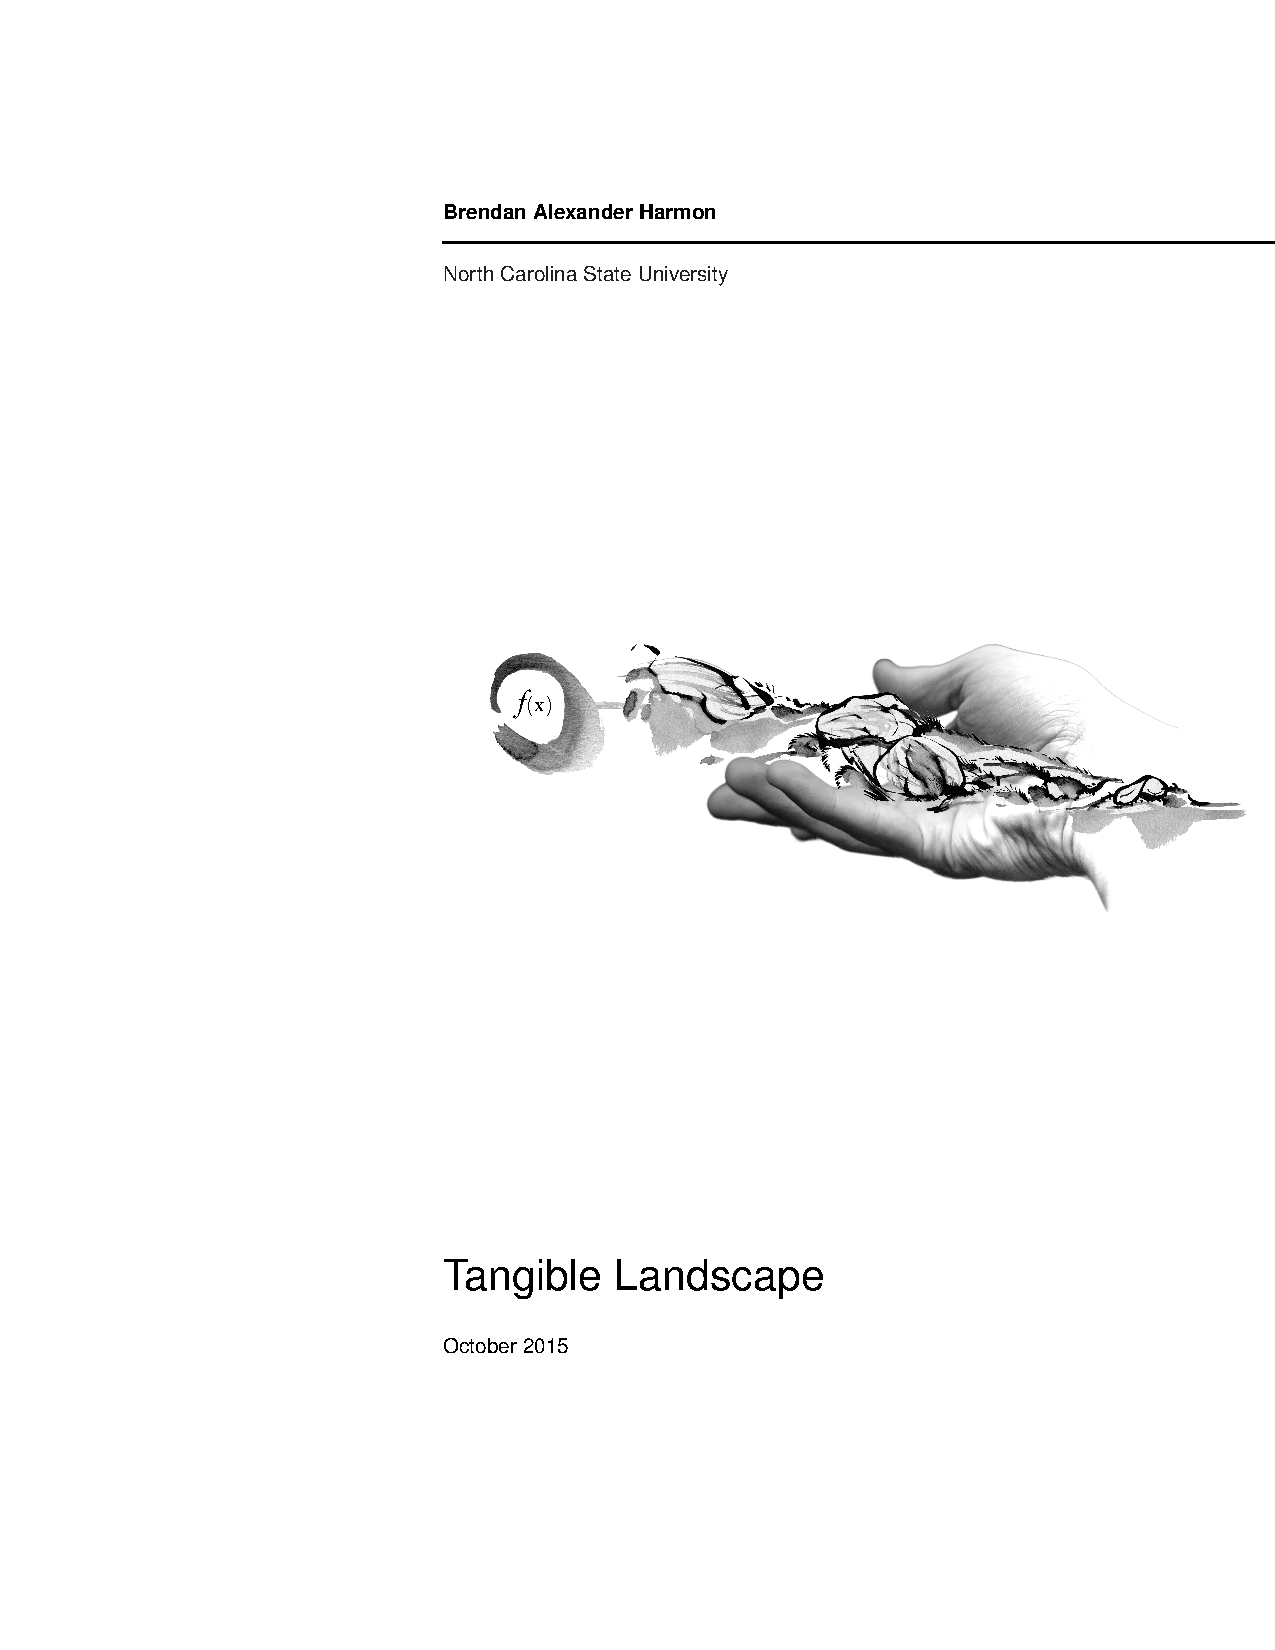
\includepdf[pages={-}]{titlepage.pdf}


%---------------------------------------------- CONTENTS ----------------------------------------------

\tableofcontents

\pagebreak

%---------------------------------------------- ABSTRACT ----------------------------------------------

\begin{abstract}

I have co-designed Tangible Landscape --
a tangible user interface 
powered by a geographic information system --
and used it to explore how 
technology mediates creativity and spatial cognition
in a rigorous experiment. 

Tangible Landscape is a continuous shape display that 
couples a malleable, interactive physical model 
of a landscape with a digital model of the landscape 
so that users can 3D sketch ideas 
and then immediately analyze them with scientific rigor. 
The physical and digital models are linked through 
a real-time cycle of 
interaction, 3D scanning, geospatial modeling, and projection. 
As we interact with a physical model of a landscape -- 
for example by sculpting the topography -- 
the changes are scanned into GRASS GIS, 
an open source geographic information system (GIS), 
for geospatial analysis and simulation 
and the resulting analytics are projected onto the physical model. 

% research issues
Tangible user interfaces are based on the premise
that embodied cognition in computing
can enhance cognitive processes.
However, the ways in which embodied cognition in computing
transform spatial thinking have not yet been rigorously studied.

% experiment
In a terrain modeling experiment 
my colleagues and I studied whether Tangible Landscape 
can enhance spatial thinking and improve spatial performance. 
We used quantitive and qualitative methods to assess 
participants' spatial performance and creative processes 
using different technologies. 
We used geospatial analytics 
such as geomorphometry and geostatistics
supplemented by semi-structured interviews and direct observation
to analyze how
visual computing with a GUI
and tangible computing with a shape display
mediate multidimensional spatial performance. 

% findings
My initial findings suggest that: 
\begin{enumerate*}[label=\bfseries \arabic*.]
\item digital sculpting via a GUI 
is unintuitive,
\item visual ambiguity 
in digital sculpting via a GUI 
leads to spatial misinterpretations,
\item shape displays like Tangible Landscape can be intuitive, 
enhance spatial performance in novel ways, 
enable rapid iteration and ideation,
and encourage creativity, and
\item different analytics encourage 
significantly different modes of spatial thinking 
and strategies for modeling. 
\end{enumerate*}

%We found that Tangible Landscape can enhance spatial performance and enable rapid iterative design processes. Tangible Landscape's cut-fill analytic enabled participants to generatively shape form and critically assess the results in an iterative cycle that significantly improved performance. Tangible Landscape's water flow simulation enabled an iterative cycle of form-finding and critical assessment that helped participants to learn how form controls process. This study shows that analytical scientific thinking can be synergistically integrated with design thinking in geodesign, enhancing rather compromising creativity.

% applications
My colleagues and I have developed applications 
for Tangible Landscape including 
stormwater management, flood control, landscape management and erosion control, 
trail planning, viewshed analysis, solar analysis, wildfire management, 
disease spread management, urban growth, and sea level rise adaption.


\end{abstract}

%---------------------------------------------- CHAPTERS ----------------------------------------------


%
\includepdf[pages={-}]{lit_rev_title.pdf}
\includepdf[pages={-}, addtotoc={1, chapter, 1, Literature review: embodied cognition in tangible computing, lit_review}]{literature_review.pdf}

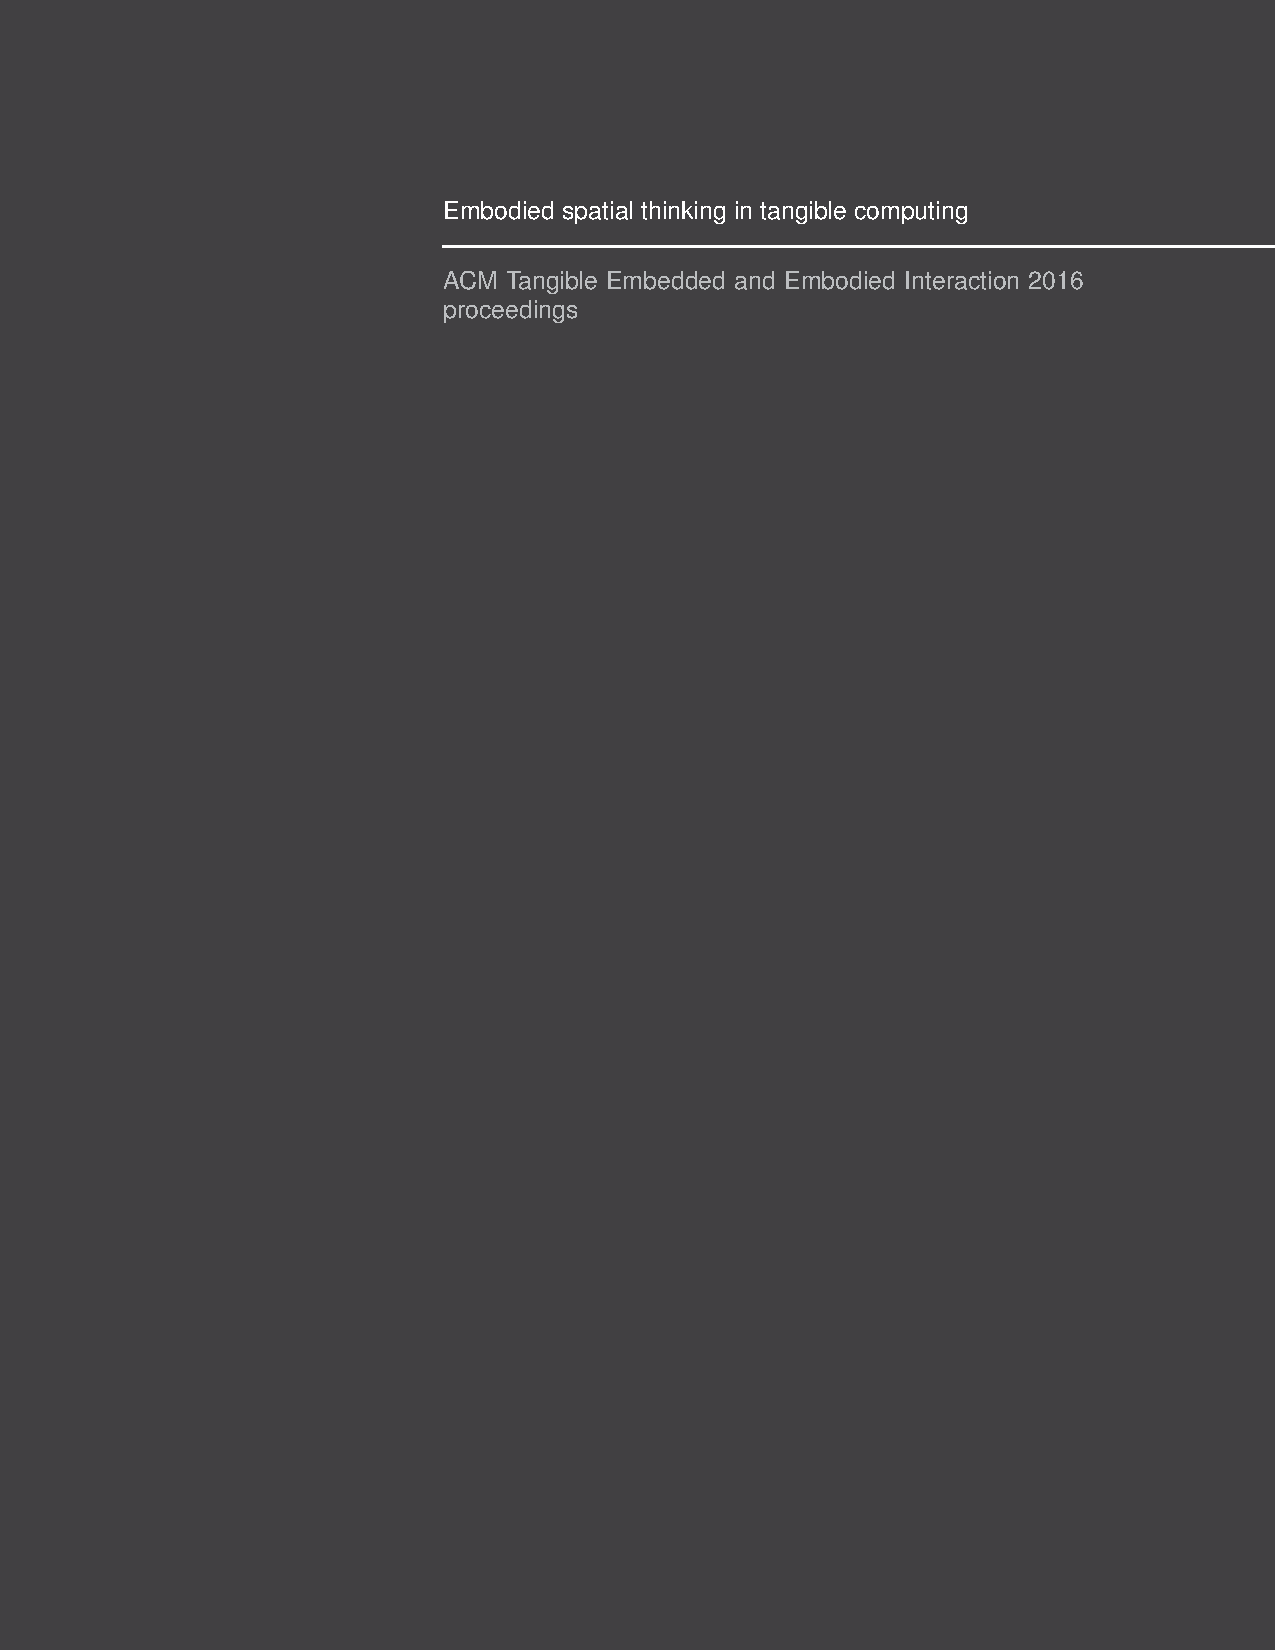
\includepdf[pages={-}]{tei_title.pdf}
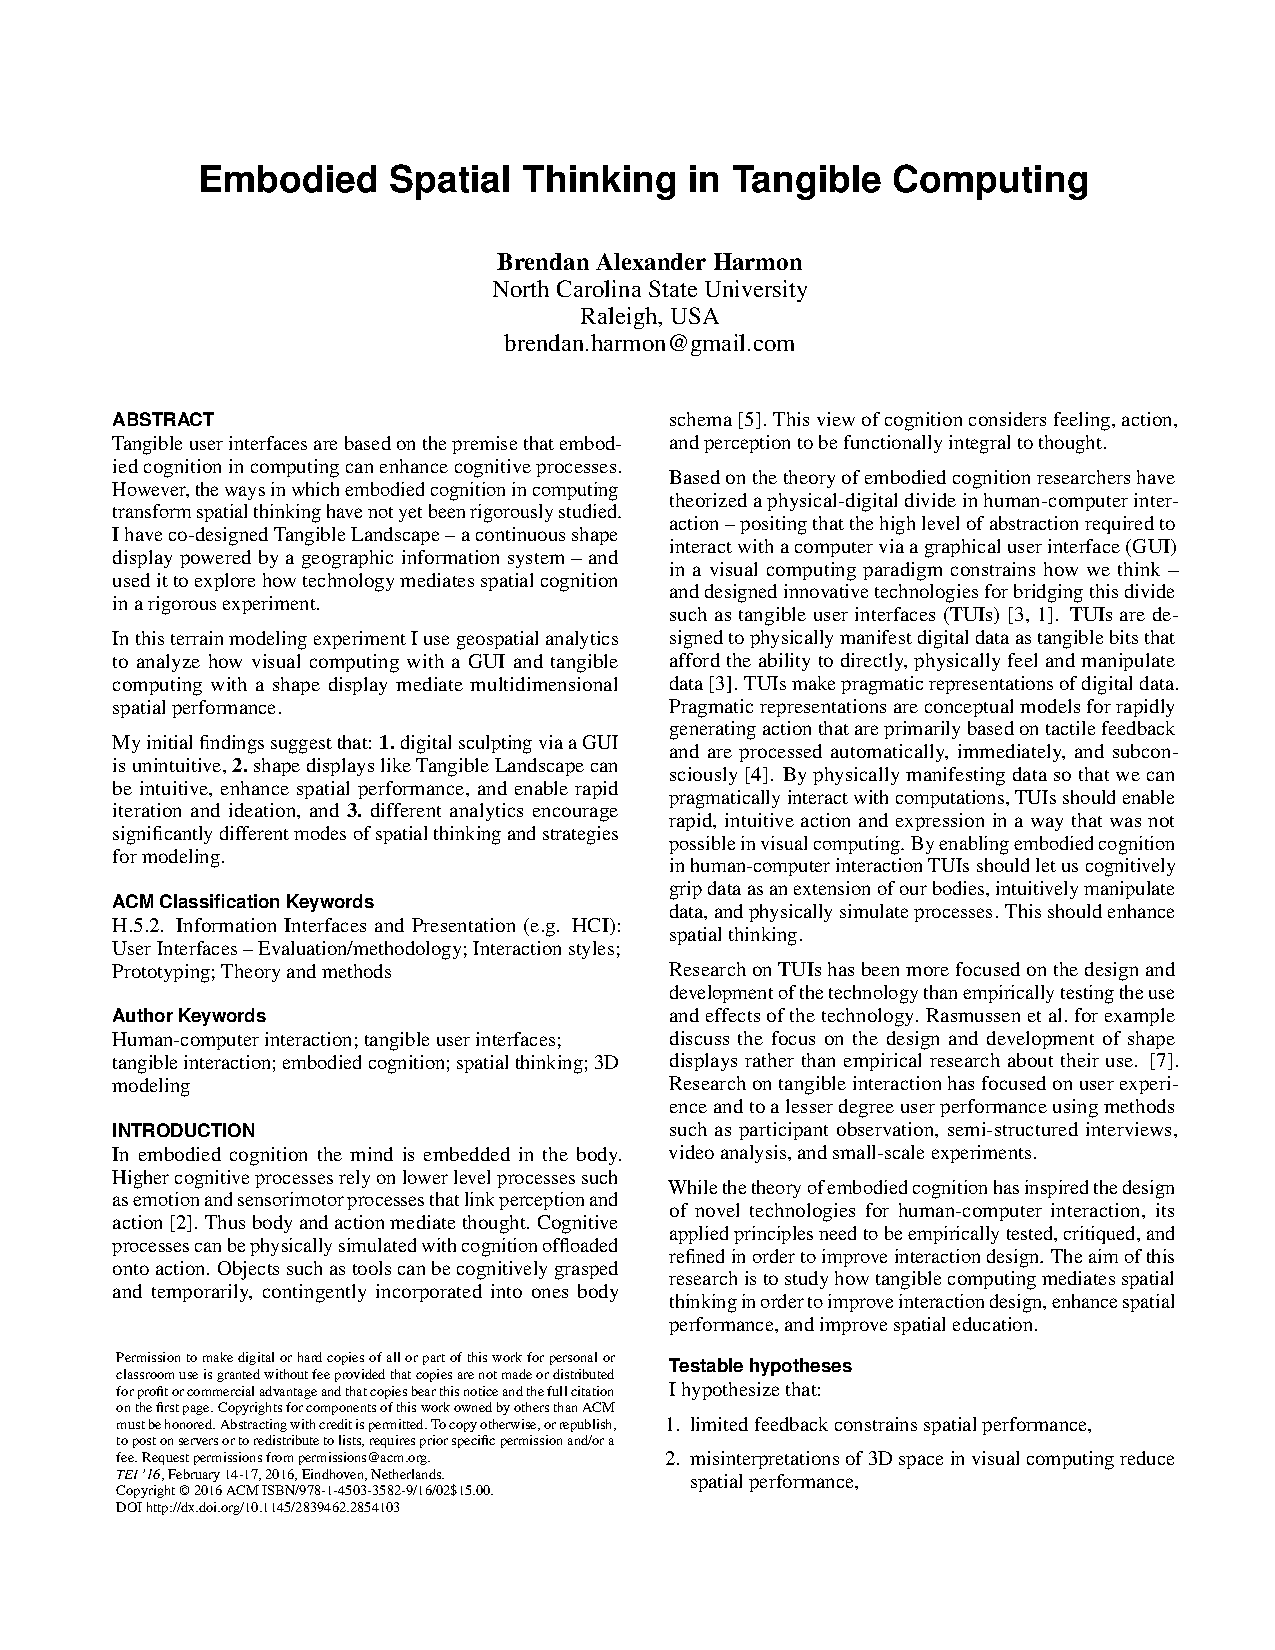
\includepdf[pages={-}, addtotoc={1, chapter, 1, Embodied spatial thinking in tangible computing, tei}]{tei_proceedings.pdf}

\includepdf[pages={-}]{tl_springer_book_title.pdf}
\includepdf[pages={-}, addtotoc={1, chapter, 1, Tangible modeling with open source GIS, book}]{tl_book.pdf}

%---------------------------------------------- BIBLIOGRAPHY ----------------------------------------------

\bibliographystyle{plainnat}
\bibliography{tangible_topography} 
\end{document}

